\section{Solver Bot}
This section will describe the physical part of the sokoban solving robot as well as introducing the controlling software in appropriate detail.
\subsection{The Robot}
The robot is built using a Lego Mindstorms kit.
from this kit two motors, three sensors and naturally, the controller is utilized.
Figures \ref{fig:robottop} and \ref{fig:robotbottom} show the robot as seen from the top and bottom, respectively.
As can be seen, two sensors, $S_1$ and $S_2$, are positioned in close proximity at the front of the robot.
These are used for line following. 

\begin{figure}[H]
	\begin{subfigure}[b]{0.49\textwidth}
		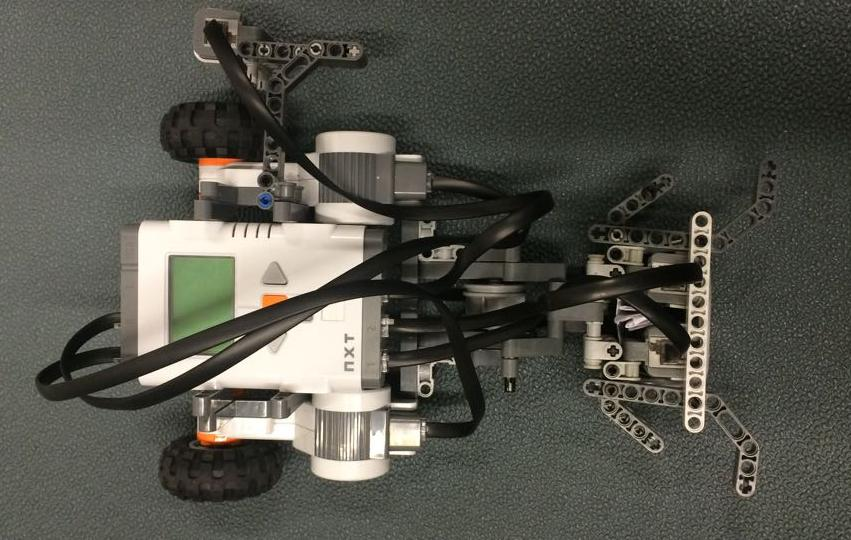
\includegraphics[angle=90, width=\linewidth]{images/robot_top}	
		\caption{The robot as seen from the top.}
		\label{fig:robottop}
	\end{subfigure}
	\begin{subfigure}[b]{0.49\textwidth}
		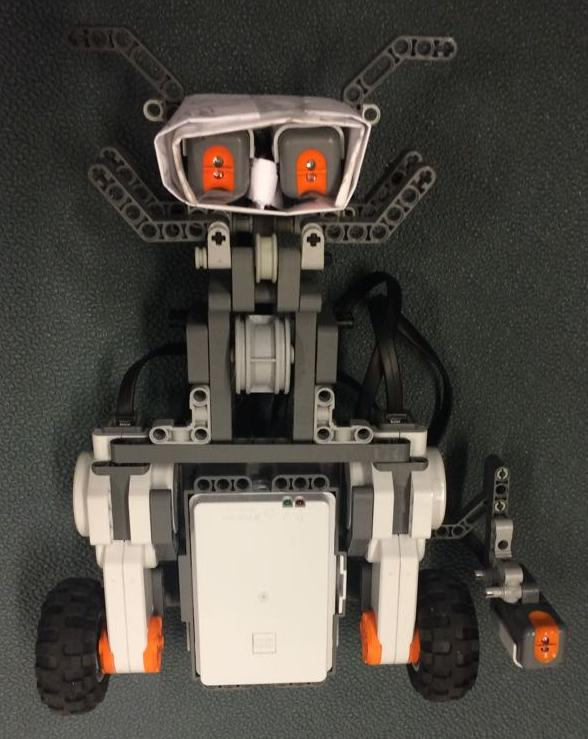
\includegraphics[width=\linewidth]{images/robot_bottom}
		\caption{The robot as seen from the bottom.}
		\label{fig:robotbottom}
	\end{subfigure}	
\end{figure}

During operation $S_1$ and $S_2$ will be positioned on either side of the line, then, if either sensor approaches the black line their value will increase.
A PID controller is then continuously attempting to keep $S_1-S_2=0$.
Should $S_1-S_2 \neq 0$ the controller will add speed to one motor and subtract from the other, depending on the sign of $S_1-S_2$. \\

At a later time the function of $S_1$ and $S_2$ was extended such that they are capable of determining when a turn is made.
At a right turn, when the right sensor reaches the black line, the turning is ended and vice versa for a left turn.
It turns out that, at appropriate speeds ($<$40\%), the delay when stopping the motors is such that the black line is again between the sensors and ready for the next command.
Unfortunately "appropriate speeds" results in a relatively slow turning speed, at least in comparison to what the robot is physically capable of.
This could be alleviated by increasing the distance between $S_1$ and $S_2$, however that would decrease the ability of the controller to stay directly on the line, a trait that is desirable when trying to keep the cans as close to the intersection as possible.\\

The final sensor, $S_3$, is used exclusively to detect when an intersection has been reached.
It is important that the sensor is positioned at the wheel base such that a turn is made as closely to the intersection as possible.\\

The design of the line following and the intersection detection both impose constraints on the maximum speed that would still allow for robust operation.
One may be tempted to increase the speed of the motors to 100\%, however in the case of the line follower this would effectively result in the controller only being able to subtract speed from one motor. 
Adding speed would have little effect when already at 100\%.
In the case of intersection detection, it turns out that the inertia of the robot carries it too far from the intersection to reliably turn and be able to then follow the line.

\subsection{Interpretation of the Path}
The solution given to the sokoban map shows the solution in terms of moves on the map itself.
The robot, however, would never drive left, it would turn left and then drive forward.
For this reason it was decided to implement only three functions to create movement:
\begin{itemize}
	\item \texttt{left(): } turns the robot 90$^\circ$ to the left.
	\item \texttt{right(): } turns the robot 90$^\circ$ to the right.
	\item \texttt{forward(): } moves the robot forwards to the next intersection.
\end{itemize}
Using this method means that the robot must know its orientation relative to the map at all times. 
This is done simply by having a variable, \texttt{orientation}, that can take the values 0-3.
In this implementation: 0:up, 1:left, 2:down, 3:right.
The \texttt{left()} function adds one while \texttt{right()} subtracts one when called.
Should \texttt{orientation} over- or under-flow it will simply wrap around.\\

A slight modification of \texttt{forward()} was necessary in order to properly push a can.
The function \texttt{push()} calls \texttt{forward()} and then continues driving forwards for 150ms and then reverses till an intersection is detection.\\

Following the solution is now a matter of calling these three+one functions in the appropriate order, e.g, if $\text{\texttt{orientation}=1}$ and the next command is 'r', \texttt{left()} is called twice followed by a call to \texttt{forward()}.

\subsection{Performance measuring}
In order to quantify the performance of the robot two test were performed. One test, perhaps obviously, was to solve the sokoban. 
The robot is capable of solving the sokoban in 3:38 minutes. 
In an attempt to measure the robustness of the robot it was set to drive in a figure 8 10$\times$5 times. 
Each figure 8 requires a total of 16 commands, resulting in a total of 800 commands executed.
The robot managed this test with no faults.
